\section{问题分析}

  \subsection{问题 1:我国能源结构分析}

    我们将煤炭、石油、天然气和一次电力及其他等能源占能源消费总量的比重,按时间序列作出折线图(见图 \ref{fig:nenyuanxiaofeibizhong})。
    \begin{figure}[hb]
      \centering
      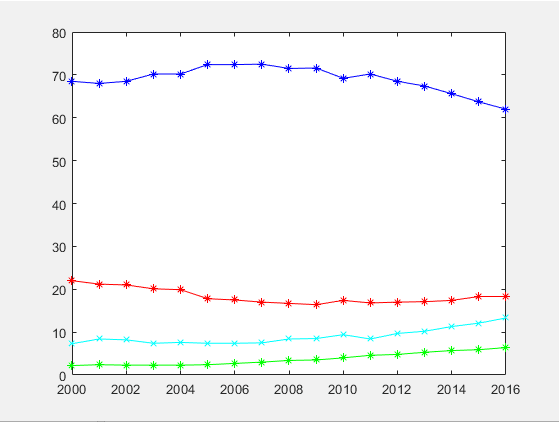
\includegraphics[scale=0.6]{figures/fig1.png}
      \captionsetup{format=hang}
      \caption[煤炭、石油、天然气和一次电力及其他等能源占能源消费总量的比重]{蓝色曲线为煤炭占总能源的比例,红色为石油,绿色为天然气,青色为一次电力及其他能源。}
      \label{fig:nenyuanxiaofeibizhong}
    \end{figure}

    由图 \ref{fig:nenyuanxiaofeibizhong} ,沿 $y$ 轴可以分析出以下几点:
    \begin{enumerate}
      \item 煤炭消费占我国能源消费的首要地位,其比例始终居于 $60\%$ 之上。
      \item 石油消费为最主要的辅助能源,其比例一直在 $20\%$ 附近。
      \item 一次电力能源与天然气在总能源中的比例相对较低,大体上低于 $10\%$ 。
    \end{enumerate}

    再沿时间轴可以分析出:
    \begin{enumerate}
      \item 煤炭消费在波动中整体呈现缓步下降趋势,但仍然占据我国能源消费的首要地位。
      \item 石油消费在参考年限中呈稳定趋势,略有波动和下滑。但与一次电力及其他的距离不断拉近。
      \item 一次电力及其他能源和天然气能源消费是呈逐年上升趋势,且天然气的上升速度随年份增加而增加。但所占比例仍然不足。
    \end{enumerate}

    \subsubsection{总结}
    我国的能源消费结构始终为以煤炭消费为主导地位,并以石油消费为主要辅助消费,但也存在天然气、一次电力及其他能源等能源占据市场。能源消费市场呈现 “一超多强” 局面。
    
    天然气和一次电力这样的清洁能源与石油、煤炭消费所占的比重不断拉近,但仍未占据可观消费比例。这说明我国的能源消费结构在不断优化的过程中还有很大的发展空间。

  \subsection{问题 2:碳排放预测模型}

    \subsubsection{碳排放影响因素分析}
      为建立模型,需要对碳排放的影响因素进行分析。根据有关文献,碳排放影响因素一般包括:
      \begin{enumerate}
        \item 人口因素;
        \item 城镇化率;
        \item 经济发展水平:人均 $GDP$ 或者消除价格波动影响的国内生产总值;
        \item 人均碳排放量;
        \item 能源消费强度:能源消费量与 $GDP$ 之比;
        \item 能源消费结构:各种能源所占比例,可以用煤炭比例来表示;
        \item 产业结构:三类产业占比,可以用第二产业占比表示;
        \item 国际贸易:出口额占 $GDP$ 比重。
      \end{enumerate}
      我们选取% TODO 因素
      进行分析。
    
    \subsubsection{模型建立}
      我们用多云线性回归分析对上述选取的因素建立了模型。

  \subsection{问题 3:政策建议}
    参见 \hyperref[sec:zhencejianyi]{7 政策建议}。